

\chapter{Orbits}



%\section{Orbits}\label{2.1}
One crucial topic that anyone working with satellites needs to understand is orbits and their characteristics. An orbit is the \textbf{gravitationally curved path of an object around a center of mass}. Examples of orbits can be the Earth around the Sun or artificial satellites around the Earth.

This section will cover the elements that describe and define an orbit, how it is represented on a map and in which way the elements that define a particular orbit can be delivered so they can be used by a computer.


\section{Kepler's Laws}\label{2.1}
Planetary movements were first mathematically defined by the German mathematician, astronomer and astrologer Johannes Kepler in the 17th century. He concentrated his observations into three simple laws\citep{SSEng}:
\begin{itemize}

\item The orbit of each planet is an ellipse with the Sun occupying one focus.
\item The line joining the Sun to a planet sweeps out equal areas in equal intervals of time.
\item A planet's orbital period is proportional to the mean distance between the Sun and the planet, raised to the power of 3/2.
\end{itemize} 

These laws apply to every celestial body. When analysing to bodies, if one is much bigger than the other, it conforms the "two-body problem". It assumes that both bodies are spherical and they are modelled as if they were point particles. This means that influences from any third body are discarded. The analysis of hits problem has resulted in six elements that completely define an orbit, which will be explained in the next section.


\pagebreak
\section{Classical Orbital Elements}\label{2.2}
The Classical Orbital Elements are six and uniquely identify an orbit. They also can be used to predict future positions.\cite{IntAstr}

The first two elements, the orbit's size and shape are defined based on a 2D representation on an ellipse (Figure \ref{f2.1}).

\begin{figure}[H]
\centerline{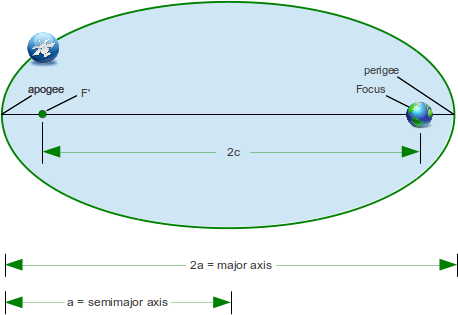
\includegraphics[width=0.7\textwidth]{images/Ellipse.png}}
\caption{Semimajor Axis}
\label{f2.1}
\end{figure}

\begin{itemize}
\item The \emph{semimajor axis} ($a$) is one half the distance across the long axis of the orbit, and it represents the orbit's size.
\item The \emph{eccentricity} represents the shape of the orbit. It describes how much the ellipse is elongated compared to a circle. Based on the latter, the orbit can have the following shapes, as shown in Figure \ref{f2.2}

\begin{figure}[H]
\centerline{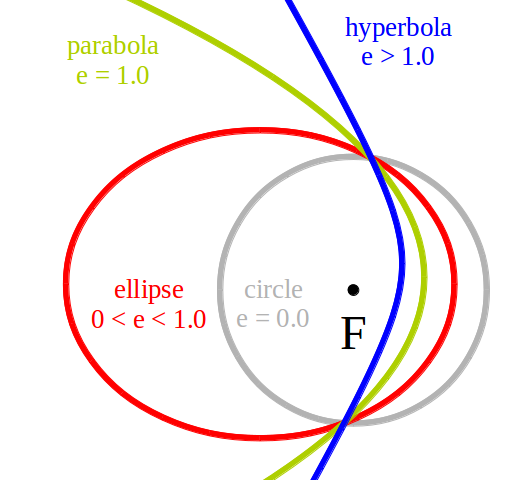
\includegraphics[scale=0.35]{images/Eccentricity.png}}
\caption{Eccentricity}
\label{f2.2}
\end{figure}

\end{itemize}


Before jumping onto the next Orbital Elements it is necessary to point out that the Geocentric-equatorial Coordinate System will be used. It is now a 3D representation, where the fundamental plane is Earth's equatorial plane and the principal direction is in the vernal equinox direction.

The following orbital elements define the orientation of the orbital plane:

\begin{itemize}
\item The inclination ($i$) describes the tilt of the orbital plane with respect to the reference plane. It is measured at the ascending node. This is, where the orbit crosses with the reference plain when moving upwards.
\item The right ascension of the ascending node ($\Omega$) represents the angle between the principal direction and the point where the orbital plane crosses the reference plane from south to north measured eastward. 
\end{itemize}

Based on this two elements, the orbits can be classified as shown in Table

\begin{table}[h]
\centering
    \begin{tabular}{| c | c | c |}
    \hline
    \textbf{Inclination} & \textbf{Orbital Type} & \textbf{Diagram}\\
     \hline
    0$^\circ$ or 180$^\circ$ & Equatorial & 
\raisebox{-\totalheight}{
\includegraphics[scale=0.5]{images/EquatorialOrbit.png}}\\ 
    \hline
\end{tabular}
  \caption{Types of Orbits and Their Inclination \cite{IntAstr}.}
  \label{Table3.1}
\end{table}